\documentclass[groupedaddress,rmp,amsmath,amssymb,bibnotes,altaffilletter,twocolumn]{revtex4-1}

%Please change this with your Unidoc number!
\newcommand{\docno}{867-5309}

\usepackage{lineno}
\usepackage{longtable}  
\usepackage{graphicx}
\usepackage{amsmath,amssymb,bbold,bm}
\usepackage{epstopdf}
\usepackage{xcolor}
\usepackage{lipsum}
\definecolor{blue}{RGB}{50,0,255}
\definecolor{orange}{RGB}{255,128,0}
\colorlet{blueh}{blue!30}
\usepackage{fancyhdr}
\fancypagestyle{uniheader}
{
\fancyhf{}% Clear all headers/footers
\fancyhead[L]{Unidoc \#M-TECHDOCUNI-\docno}% Header Centred
  \fancyfoot[C]{-\thepage-}% Footer Centred
  \renewcommand{\headrulewidth}{2pt}% 
  \renewcommand{\headheight}{52pt}% 
  \renewcommand{\headrule}{\hbox to\headwidth{%
    \color{orange}\leaders\hrule height \headrulewidth\hfill}}
  \renewcommand{\footrulewidth}{0pt}% No footer rule
  \rhead{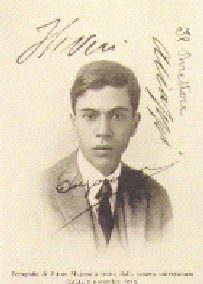
\includegraphics[width=1cm]{figs/MJD}}
}

\usepackage{soul}
\newcommand{\hlc}[2][yellow]{ {\sethlcolor{#1} \hl{#2}} }

\begin{document}

\def\nuc#1#2{${}^{#1}$#2}
\def\mee{$\langle m_{\beta\beta} \rangle$}
\def\mnu{$m_{\nu}$}
\def\ml{$m_{lightest}$}
\def\gnu{$\langle g_{\nu,\chi}\rangle$}
\def\mmod{$\| \langle m_{\beta\beta} \rangle \|$}
\def\mb{$\langle m_{\beta} \rangle$}
\def\BBz{$\beta\beta(0\nu)$}
\def\BBm{$\beta\beta(0\nu,\chi)$}
\def\BBt{$\beta\beta(2\nu)$}
\def\nonubb{$\beta\beta(0\nu)$}
\def\twonubb{$\beta\beta(2\nu)$}
\def\BB{$\beta\beta$}
\def\Mz{$M_{0\nu}$}
\def\Mt{$M_{2\nu}$}
\def\MzG{$M^{GT}_{0\nu}$}           %Gamov-Teller
\def\MzF{$M^{F}_{0\nu}$}                %Fermi
\def\MtG{$M^{GT}_{2\nu}$}           %Gamov-Teller
\def\MtF{$M^{F}_{2\nu}$}                %Fermi
\def\Gz{$G_{0\nu}$}					%phase space factor for 0nu
\def\Tz{$T^{0\nu}_{1/2}$}
\def\Tt{$T^{2\nu}_{1/2}$}
\def\Tc{$T^{0\nu\,\chi}_{1/2}$}
\def\Rz{$\Gamma_{0\nu}$}            %0 nu decay rate
\def\Rt{$\Gamma_{2\nu}$}            %2 nu decay rateq
\def\ms{$\delta m_{\rm sol}^{2}$}
\def\ma{$\delta m_{\rm atm}^{2}$}
\def\mot{$\delta m_{12}^{2}$}
\def\mtt{$\delta m_{23}^{2}$}
\def\ts{$\theta_{\rm sol}$}
\def\ta{$\theta_{\rm atm}$}
\def\ttwo{$\theta_{12}$}
\def\tot{$\theta_{13}$}
\def\gpp{$g_{pp}$}                  % the g_pp of QRPA fame
\def\gA{$g_{A}$}                  % the Axial Vector coupling constant
\def\qval{$Q_{\beta\beta}$}                 % The Q-value
\def\be{\begin{equation}}
\def\ee{\end{equation}}
\def\cpKkgy{cnts/(keV kg y)}
\def\cpKkgd{cnts/(keV kg d)}
\def\cpRty{cnts/(ROI t y)}
\def\onecpRty{1~cnt/(ROI t y)}
\def\threecpRty{3~cnts/(ROI t y)}
\def\ppc{P-PC}                          % P-type Point Contact
\def\nsc{N-SC}                          % N-type Segmented Contact
\def\cosixty{$^{60}Co$}
\def\baott{$^{133}Ba$}
\def\thttt{$^{232}\mathrm{Th}$}
\def\thtte{$^{228}\mathrm{Th}$}
\def\utte{$^{238}\mathrm{U}$}
\def\mubqkg{$\mu\mathrm{Bq/kg}$}
\def\cusulfate{$\mathrm{CuSO}_4$}
\def\MJ{{\sc Majorana}}             %Majorana project name
\def\DEM{{\sc Demonstrator}}             %Demonstrator in small caps
\def\MJDEMbf{\bfseries{\scshape{Majorana Demonstrator}}}
\def\MJbf{\bfseries{\scshape{Majorana}}}
\def\MJDEMit{\itshape{\scshape{Majorana Demonstrator}}}
\newcommand{\Gerda}{GERDA}
\newcommand{\GF}{\textsc{Geant4}}
\newcommand{\MaGe}{\textsc{MaGe}}
\def\Higgs{Hi$\gamma\gamma$s}


\newcommand{\bhsu}{Black Hills State University, Spearfish, SD, USA}
\newcommand{\duke}{Duke University, Durham, NC, USA}
\newcommand{\kurchatov}{National Research Center “Kurchatov Institute” Institute for Theoretical and Experimental Physics, Moscow, Russia}
\newcommand{\jinr}{Joint Institute for Nuclear Research, Dubna, Russia}
\newcommand{\lanl}{Los Alamos National Laboratory, Los Alamos, NM, USA}
\newcommand{\lbnl}{Lawrence Berkeley National Laboratory, Berkeley, CA ,USA}
\newcommand{\ncsu}{North Carolina State University, Raleigh, NC, USA}
\newcommand{\ornl}{Oak Ridge National Laboratory, Oak Ridge, TN, USA}
\newcommand{\rcnp}{Research Center for Nuclear Physics, Osaka University, Ibaraki, Japan}
\newcommand{\pnnl}{Pacific Northwest National Laboratory, Richland, WA, USA}
\newcommand{\queens}{Queen’s University, Kingston, ON, Canada}
\newcommand{\sdsmt}{South Dakota School of Mines and Technology, Rapid City, SD, USA}
\newcommand{\tunl}{Triangle Universities Nuclear Laboratory, Durham, NC, USA}
\newcommand{\ttu}{Tennessee Tech University, Cookeville, TN, USA}
\newcommand{\unc}{University of North Carolina at Chapel Hill, Chapel Hill, NC, USA}
\newcommand{\usc}{University of South Carolina, Columbia, SC, USA}
\newcommand{\usd}{University of South Dakota, Vermillion, SD, USA}
\newcommand{\utk}{University of Tennessee, Knoxville, TN, USA}
\newcommand{\cenpa}{Center for Experimental Nuclear Physics and Astrophysics, University of Washington, Seattle, WA, USA}
\newcommand{\ucBerk}{University of California, Berkeley, USA}

%Update your title, name and affiliation
\title{Validation of the Pulse Shape Simulation Tools}
%These have to be in order in which they appear for the authors:
\affiliation{\unc}
\affiliation{\tunl}

\author{C.M.~O'Shaughnessy}\affiliation{\unc}\affiliation{\tunl}
\author{J.~Rager}\affiliation{\unc}\affiliation{\tunl}

			

%%%%%% Replace the abstract here %%%%%%
\begin{abstract}
  The waveform generation for \MJ~uses the fieldgen and siggen tools. While these are fairly throughly validated by both the use in GRETINA and by the WF-fitting routines that have also been developed. We must be certain that no systematic effects enter an analysis that utilizes these simulations for estimation of the systematic effects of PSAs.  
\end{abstract}

%%%%%% Formatting, don't change these %%%%%%
\pagestyle{uniheader}

\date{\today}
\maketitle
\thispagestyle{uniheader}
\tableofcontents
%%%%%%%%%%%%

%%%%%% This section is the introduction, you may rename it, but please introduce the analysis topic. %%%%%%%
\section{Introduction}

In the evaluation of the various Pulse Shape Analysis (PSA) routines developed by \MJ~we intend to utilize Pulse Shape Simulations (PSS) to estimate the systematic uncertainties incurred. To do this with confidence we must be sure there is no systematic difference between the simulated waveforms and waveforms with data within the measure being addressed. 

To perform the validation a number of datasets are used. We use a source of collimated \baott~as a clean source of surface events with 81~keV. These data are expected to generate waveforms with a very characteristic pulse shape distribution. The distribution of single site events in the single-escape peak (SEP) and double-escape peak (DEP) are also known to have unique distributions and therefore calibration data from a \thtte~source is also utilized.

%%%%%% This section should describe the signature or the methods you are trying to take advantage of %%%%%%
\section{Validation techniques}

\subsection{Collimated \baott}
A series of scans were taken using a collimated \baott~button source. The lead collimation was XXX~mm in diameter by XXX~mm long and was situated XX mm from the surface of the STC, resulting in a distance of XX-XX~mm from the detector. To clean the dataset from backgrounds a coincidence cut is applied. This is a coincidence between 81~keV gammas in the detector vs 356~keV gammas in the NaI detector. Since these gammas occur in coincidence X\%, this results in a XX\% reduction in background events.

Gammas with an energy of 81~keV have a mean free path of XX mm in germanium. This results in a spot size of roughy XX by XX by XX on the surface of the detector. Given this very specific position distribution of events on the detector, the distribution of waveforms shapes are also specific to the collimation geometry. Waveform risetime is one of the more sensitive parameters to the position. By parameterizing the risetime distribution, peak position, width, etc. we can compare simulation to a z-scan of a detector. 

Additionally we can make use of the superpulse classes to characterize the distributions of pulse shapes from collimated data. By generating a library of superulses with a variety of chi-square thresholds we expect the distribution of shapes to be similar and therefore the frequency of similar waveforms to also be similar. Adding waveforms from simulation to the superpulse library generated by data should only scale in magnitude if the distributions are similar. 

Another way to utilize superpulses is to create a single superpulse of all events from a run after A/E cut for single site events. This will average the waveform shape in non-physical ways, however if the distribution of events are similar the averaging should be similar for data and simulation. 

\subsection{Calibration Data}

Other data samples that have a specific position distribution depending on the detector geometry include the DEP and SEP events from pair production. These are more likely to occur at the detector surfaces and corners. By fitting the simulated wavforms to data we can estimate the most likely position of the event. This should lead to the distribution of events that are similar to those simulated for calibrations of the same detectors.

\subsection{\cosixty~Data}

Since fitting the low energy collimated data that have fairly well known position distributions does not yield high precision fits, one can also consider using \cosixty data from a characterization scan. Collimation of the \cosixty source does not yield precision information about the position due to the increased mean free path of higher energy gammas, it also leads to events with degraded energy and produces an energy spectrum with linewidths washed out. We will first simulate the collimation and design an optimized collimator to minimize these effects. An alternative could be to use a gross collimation and an NaI detector to measure compton scattered events. At high angles most of the energies are deposited and one can utilize the kinematics to reconstruct the vertex position.  

\subsection{\Higgs~scans}

Similar to collimated \cosixty~it is possible that we could operated the detector at the \Higgs~facility where we can select the energy and collimate the beam to perform high energy scans of the detector. This will provide data that can be fit using the WF fitting tools and given the specific geometry we would be able to use these data to determine the systematics uncertainty in the fir positions by comparing with a simulated model of the \Higgs~source. 

\section{A test of our methods}

\hlc[blueh]{Validate your techniques. Since this is a unidoc we want lots of detail here. What did you do to convince yourself the analysis is correct? Did you benchmark your analysis? How did you do this? How does it compare to previous analyses?
}
%
\begin{equation}
\frac{d\Gamma(E)}{dE} = \frac{\alpha \lambda}{\pi a^2 m^2_e E},
\label{eqn:rate1}
\end{equation}
%
\lipsum[2-2] 

\begin{equation}
\lambda < \frac{R_0}{k_T N_{Ge} N_e \gamma}.
\label{eqn:rateExpUnits2}
\end{equation}
%
\lipsum[3-3]

%%%%%% In this section you should validate your techniques. %%%%%% 

The result of our $R_0/E$ fit is shown in Fig.~\ref{fig:IGEXfit} and the resulting value for $R_0=1.38$ /(kg k) agrees very will with the previous work. 

\begin{figure}[t]
 \centering
 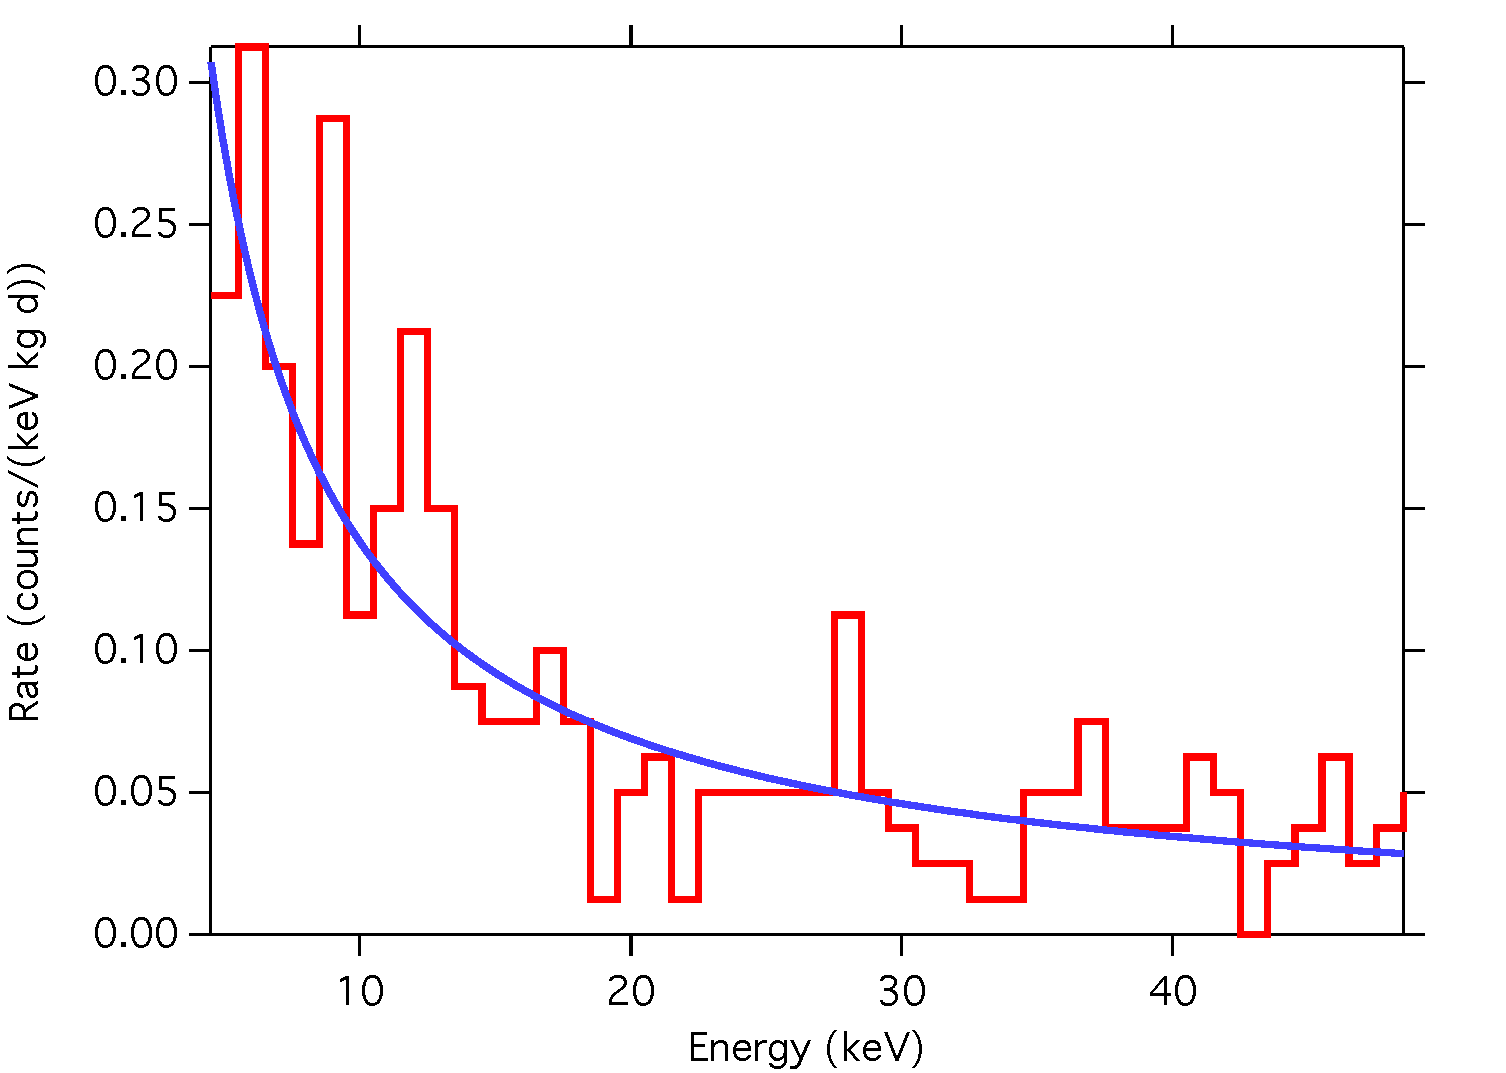
\includegraphics[width=1.0\columnwidth]{figs/IGEXfit.pdf}
 \caption{The energy spectrum from IGEX~\cite{Morales2002} with a fit to the function $R_0/E$ with the result $R_0=1.38$ counts/(kg d).}
 \label{fig:IGEXfit}
\end{figure}


To convert $R_0$ into a limit on $\lambda$,
%
\begin{eqnarray}
\lambda & < & \frac{1.38 \mbox{/kg d}}{(86400 \mbox{ s/d}) (7.96\times10^{24} \mbox{/kg}) (22) (3.46\times10^{-14})}\nonumber  \\ 
 & < & 2.6\times10^{-18} \mbox{ /s}.
\label{eqn:LamLimit}
\end{eqnarray}
%
This result agrees with the previous work.

\lipsum[3-3]

%%%%%% This is a results section %%%%%%
\section{\MJ\ Analysis}
\hlc[blueh]{This is the results, you applied the methods described previously to the data described previously and these are the results you get. First what are they with no interpretation. Next do you have an interpretation of these results? Is future work required? What worked? What didn't?
}

\lipsum[4-4]

%%%%%% Any additional considerations for a publication %%%%%%
\section{Journal Thoughts}
\hlc[blueh]{How were previous results published? What journals make sense to present these results in?}

\bibliography{unidoc}




\end{document}
